\documentclass[11pt,a4paper]{article}
\usepackage[T1]{fontenc}
\usepackage{lmodern}
\usepackage[spanish]{babel}
\usepackage[margin=2.5cm]{geometry}
\usepackage{booktabs,tabularx,graphicx,hyperref,enumitem,parskip}
\hypersetup{hidelinks}
\setlength{\parskip}{0.6em}
\begin{document}

{\LARGE\bfseries Proyecto final: clasificación visual de productos para Lokora\par}\vspace{0.4em}
\noindent \textbf{Avance II (R2-A3-S12). Pipeline}\par
\noindent Universidad de Cundinamarca. Posgrado. Aplicaciones en Deep Learning (608145)\par
\noindent Docente: Wilson Mauro Rojas Reales\par
\noindent Estudiante: Harold Duque (trabajo individual)\par
\noindent Fecha: 17 de noviembre de 2026\par
\section*{Resumen}
\noindent Este documento describe el pipeline del proyecto: de dónde provienen los datos, cómo se preprocesan y cómo se organiza el repositorio. El problema y el diseño de la solución se encuentran en el Avance I. Los resultados del entrenamiento de la red se presentan en el Avance III.\par
\section*{Avance II. Pipeline}
\subsection*{5. Diagrama del flujo de datos}
\noindent La figura 2 muestra el flujo desde las fotografías hasta el uso propuesto, con los artefactos que conserva cada ejecución.\par
\begin{figure}[htbp]\centering
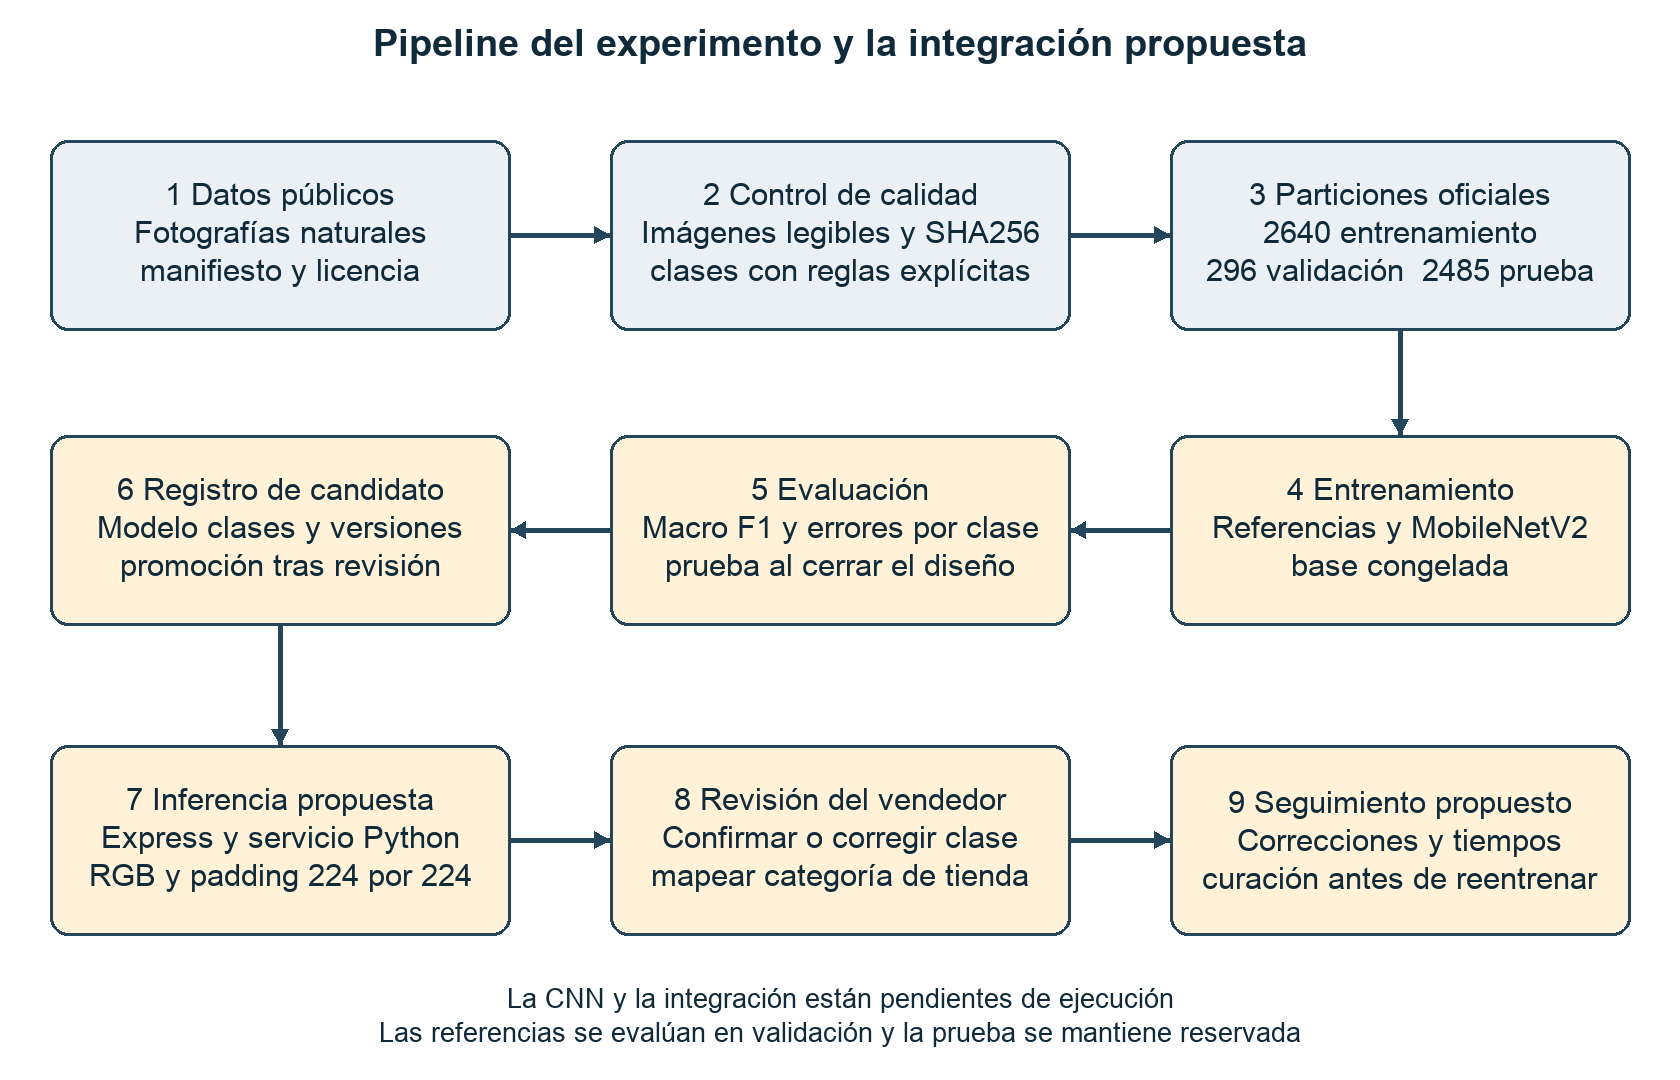
\includegraphics[width=0.92\textwidth]{figuras/pipeline_lokora.png}
{\small Figura 2. Pipeline del experimento y la integración propuesta\par}
\end{figure}
\subsection*{6. Recolección de datos y fuentes}
\begin{center}\small
\begin{tabularx}{\textwidth}{XXXX}
\toprule
\textbf{Fuente} & \textbf{Contenido} & \textbf{Licencia} & \textbf{Estado} \\
\midrule
Grocery Store Dataset (Klasson et al., 2019). \url{https://github.com/marcusklasson/GroceryStoreDataset} & Fotografías de frutas, verduras y productos envasados con listas oficiales de entrenamiento, validación y prueba & MIT & Descargado y preparado \\
Fotografías propias de comercios de Lokora & Productos reales con categoría confirmada & Propia & Pendiente de recolección \\
Correcciones del vendedor & Sugerencia frente a categoría final & Propia & Se generará en el piloto \\
\bottomrule
\end{tabularx}
\end{center}
\noindent Se usan solo las fotografías naturales. Las imágenes icónicas y las descripciones del conjunto quedan fuera. Las carpetas Fruit, Vegetables y Packages se mapean a \texttt{frutas}, \texttt{verduras} y \texttt{envasados}; el tomate sigue la convención del conjunto y se etiqueta como verdura.\par
\begin{center}\small
\begin{tabularx}{\textwidth}{>{\raggedright\arraybackslash}p{0.28\textwidth}>{\raggedleft\arraybackslash}p{0.193\textwidth}>{\raggedleft\arraybackslash}p{0.193\textwidth}>{\raggedleft\arraybackslash}p{0.193\textwidth}}
\toprule
\textbf{Categoría} & \textbf{Entrenamiento} & \textbf{Validación} & \textbf{Prueba} \\
\midrule
Envasados & 864 & 100 & 781 \\
Frutas & 1.142 & 111 & 1.117 \\
Verduras & 634 & 85 & 587 \\
\textbf{Total} & \textbf{2.640} & \textbf{296} & \textbf{2.485} \\
\bottomrule
\end{tabularx}
\end{center}
\subsection*{7. Preprocesamiento}
\begin{enumerate}[nosep]
\item Lectura respetando la orientación EXIF y conversión a RGB.
\item Redimensión con relleno a 224 $\times$ 224 píxeles.
\item Escalado de 0--255 a -1--1, aplicado una sola vez dentro del modelo.
\item Aumento de datos solo durante el entrenamiento.
\item Manifiesto con ruta, clase, partición oficial, fuente, licencia y SHA-256. No se encontraron duplicados exactos; esto no descarta fotos visualmente parecidas.
\end{enumerate}
\noindent \textbf{Límite de independencia.} Los metadatos no identifican el objeto físico ni la sesión de captura, así que no se puede afirmar separación por producto. Con fotos propias se agruparán por producto o sesión, de modo que un grupo quede en una sola partición.\par
\subsection*{8. Resultados disponibles al corte}
\noindent Esta sección recoge las referencias de comparación, evaluadas sobre las 296 fotografías de validación. La evaluación de MobileNetV2 y de la partición de prueba se reporta en el Avance III.\par
\begin{center}\small
\begin{tabularx}{\textwidth}{XrrX}
\toprule
\textbf{Modelo} & \textbf{Exactitud (validación)} & \textbf{Macro-F1 (validación)} & \textbf{Estado} \\
\midrule
Clase más frecuente & 0,3750 & 0,1818 & Ejecutado \\
Histograma RGB y regresión logística & 0,5304 & 0,5136 & Ejecutado \\
\bottomrule
\end{tabularx}
\end{center}
\subsection*{9. Repositorio y reproducibilidad}
\noindent Repositorio en GitHub: \url{https://github.com/HaroldDuke/lokora-clasificacion-productos}\par
\noindent El repositorio está organizado en \texttt{ml/} (código), \texttt{notebooks/}, \texttt{config/}, \texttt{datos/} (plantillas), \texttt{resultados/}, \texttt{diagramas/} y \texttt{docs/}, e incluye un README con instalación, uso y dependencias. El antecedente de la aplicación pertenece al equipo Axiom (\url{https://github.com/cataia-code/interledger-axiom-hackathon}); esta extensión es un trabajo académico individual.\par
\subsection*{10. Siguientes pasos}
\begin{center}\small
\begin{tabularx}{\textwidth}{XX}
\toprule
\textbf{Entrega} & \textbf{Contenido} \\
\midrule
23 de noviembre (Avances III y IV) & Entrenar MobileNetV2 en Colab, comparar con las referencias, analizar errores y evaluar en prueba una sola vez \\
25 de noviembre (Avance V y proyecto final) & Evaluación con fotografías propias, flujo de confirmación y medición de tiempo y correcciones \\
\bottomrule
\end{tabularx}
\end{center}
\subsection*{Referencias}
\noindent [1] Klasson, M., Zhang, C. y Kjellström, H. (2019). A Hierarchical Grocery Store Image Dataset with Visual and Semantic Labels. IEEE Winter Conference on Applications of Computer Vision (WACV). \url{https://arxiv.org/abs/1901.00711}\par
\noindent [2] Sandler, M., Howard, A., Zhu, M., Zhmoginov, A. y Chen, L.-C. (2018). MobileNetV2: Inverted Residuals and Linear Bottlenecks. CVPR. \url{https://arxiv.org/abs/1801.04381}\par
\noindent [6] Axiom. Lokora, proyecto de la hackatón Open Payments, Medellín, 16 y 17 de octubre de 2026.\par
\noindent [7] Keras. Transfer learning and fine tuning. \url{https://keras.io/guides/transfer_learning/}\par
\end{document}
